\chapter{Implementation Walkthrough}

\section{Client Implementation Path}
The \texttt{VPNClient} class orchestrates startup and forwarding. Constructor logic validates required config keys, initializes endpoint parameters, and prepares runtime state containers (socket, framer, tun interface, threads, stats).

\subsection{Startup Sequence}
The operational sequence in \texttt{start()} is clear and linear:
\begin{enumerate}[leftmargin=2em]
\item Register signal handlers for graceful shutdown.
\item Connect to server over TCP.
\item Authenticate via \texttt{authenticate\_connection(..., is\_server=False)}.
\item Initialize \texttt{PacketFramer} over connected socket.
\item Set up TUN interface and assign configured tunnel IP.
\item Start two forwarding threads.
\item Enter periodic stats loop until termination.
\end{enumerate}

\section{Server Implementation Path}
\texttt{VPNServer} mirrors client logic but adds passive listen/accept behavior. Notable server-specific details:
\begin{itemize}[leftmargin=2em]
\item Socket configured with \texttt{SO\_REUSEADDR}.
\item \texttt{listen(1)} enforces single client in MVP.
\item Accept thread performs auth before starting packet forwarding.
\end{itemize}

\section{TUN Interface Abstraction}
\texttt{TunInterface} encapsulates Linux-specific setup:
\begin{itemize}[leftmargin=2em]
\item \texttt{/dev/net/tun} is opened with read/write flags.
\item \texttt{ioctl(TUNSETIFF)} creates configured TUN device.
\item File descriptor is switched to non-blocking mode.
\item Interface IP and MTU are configured through \texttt{ip} commands.
\end{itemize}

Packet reads use \texttt{select.select} with timeout, enabling loops to stay responsive to \texttt{self.running} changes.

\section{Utilities and Shared Services}
\subsection{Config Pipeline}
\texttt{load\_config()} reads JSON and automatically decodes \texttt{key\_base64} into raw bytes for runtime crypto calls. This keeps endpoint code uncluttered and prevents repetitive decoding logic.

\subsection{Statistics}
\texttt{Stats} tracks packet and byte counters for each direction plus decrypt failures. The string representation is log-friendly and suitable for periodic heartbeat diagnostics.

\section{Error Handling Philosophy}
Implementation favors explicit exception capture by category:
\begin{itemize}[leftmargin=2em]
\item Tunnel failures raise \texttt{TunnelError}.
\item Framing/socket issues raise \texttt{ProtocolError} or socket exceptions.
\item Crypto faults raise \texttt{CryptoError} and increment failure counters.
\end{itemize}

This approach is understandable for learners because failure sources remain visible in logs and map directly to subsystem boundaries.

\section{Code Listing: Receive-Decryption-Inject Loop}
\begin{lstlisting}[style=vpnpython,caption={Data-plane receive path pattern from client/server loops}]
encrypted_packet = self.framer.recv(timeout=1.0)
if encrypted_packet is None:
    continue
packet = decrypt(encrypted_packet, self.key)
self.tun.write_packet(packet)
self.stats.record_packet_in(len(packet))
\end{lstlisting}

\section{Scripted Environment Workflows}
Implementation is supported by shell utilities to reduce manual setup burden. Scripts create namespaces, veth links, forwarding rules, DNS files, and cleanup paths. This ecosystem effectively functions as a deployment harness for demonstrations.

\begin{figure}[H]
\centering
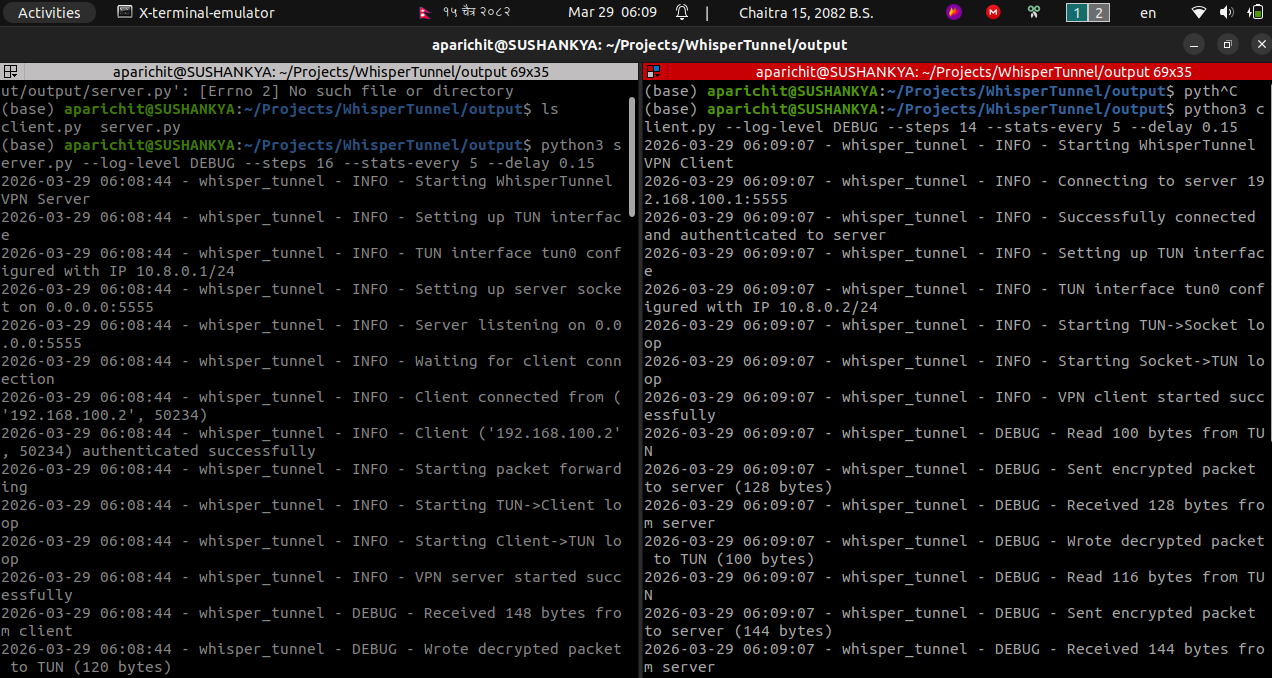
\includegraphics[width=0.95\textwidth]{figures/runtime-shapshot.png}
\caption{Runtime Snapshot of Server and Client Logs}
\label{fig:runtime-snapshot}
\end{figure}

\section{Potential Refactors for Maintainability}
Several clean refactors can improve maintainability without changing functionality:
\begin{enumerate}[leftmargin=2em]
\item Extract shared loop logic into a generic forwarding worker.
\item Add structured lifecycle state machine to reduce flag-based control.
\item Introduce dataclass-based config models with typed validation.
\item Normalize script variables and strict shell linting.
\item Replace duplicate wrapper modules with explicit import conventions.
\end{enumerate}

\section{Complexity Profile}
The implementation remains compact, with most technical complexity concentrated in three files:
\begin{itemize}[leftmargin=2em]
\item \texttt{client/client.py}
\item \texttt{server/server.py}
\item \texttt{common/tunnel.py}
\end{itemize}

This concentration is favorable for educational walkthroughs because students can understand end-to-end behavior by mastering a small subset of files.

\section{Observations on Operational Robustness}
While code pathways are clear, robustness constraints include:
\begin{itemize}[leftmargin=2em]
\item Limited reconnection behavior.
\item No backoff strategy for transient network issues.
\item Single-client server assumptions in socket acceptance.
\item Script-level variance in namespace and host execution expectations.
\end{itemize}

These constraints are expected for MVP educational systems and become roadmap candidates rather than immediate defects.
